\section{Élaboration d'un modèle de comportement dynamique lors du suivi de trajectoire}

L'objectif de cette partie est d'élaborer un modèle de comportement dynamique du système articulé lors de la dépose de bouteilles dans une caisse TSR. Pendant cette phase, le point $E$, centre de rotation du poignet par rapport au bras 3 (voir Annexe D.2), doit suivre une trajectoire rectiligne verticale pour éviter toute collision entre les bouteilles et les différentes parois de la caisse TSR. Les caractéristiques de cette trajectoire sont définies par la Figure \ref{fig:07} où le point $E$ se déplace sur le segment $\left[E_{1} E_{2}\right]$.

\begin{figure}[!h]
\centering
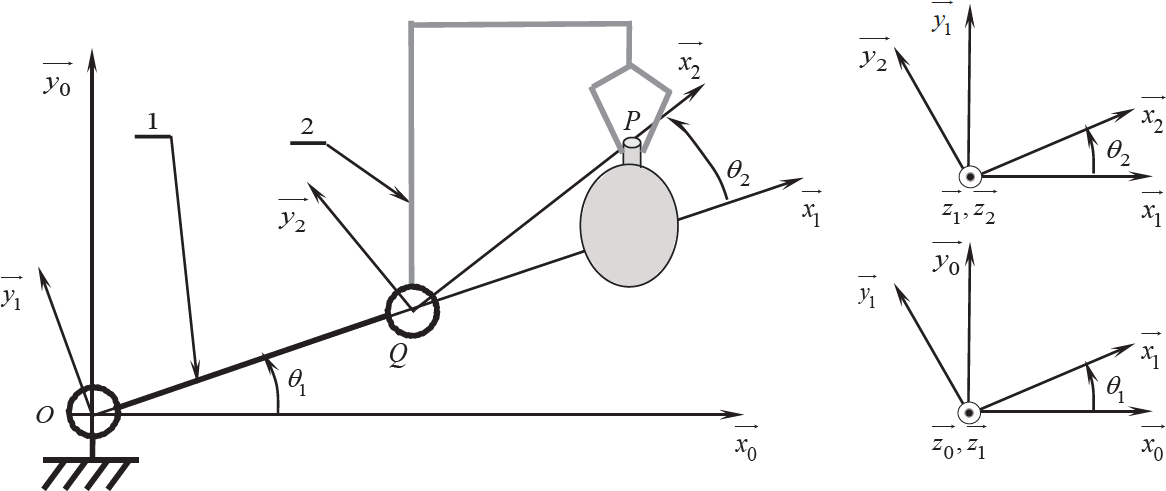
\includegraphics[width=.5\textwidth]{fig_07}
%Figure 7 - 
\caption{Configuration du robot lors de la confection de caisse TSR 504 \label{fig:07}}
\end{figure}


\subsection{Étude du système de compensation de gravité du robot}
Le robot est équipé d'un système de compensation de gravité dont on cherche à quantifier les effets lors du suivi de la trajectoire verticale $\left(E_{1} E_{2}\right)$, en fonction des charges et de leur position. Le paramétrage du robot est donné en Annexe D.2. Le système de compensation de gravité est constitué d'un vérin (pièces 7 et 8) de longueur $\lambda(t)$ et muni d'un ressort dont la longueur à vide sera notée $\lambda_{0}$ pour l'étude.

On donne $\torseurstat{T}{8}{2}$, le torseur modélisant l'action du système de compensation sur le bras 2 .

La relation entre $F_{\text {res }}$ et $\lambda$ est supposée linéaire avec $F_{\text {res }}=k_{r} \cdot\left(\lambda-\lambda_{0}\right), \quad \torseurstat{T}{8}{2}=\left\{\begin{array}{c}\vec{R}_{8 \rightarrow 2}=-F_{\text {res }} \cdot \vec{x}_{7} \\ k_{r}=200 \mathrm{~N} \cdot \mathrm{mm}^{-1} \text { et } \lambda_{0}=405 \mathrm{~mm} .\end{array}\right\}$

\question{\label{q:11} Donner l'expression du couple $C_{\text {res }}$ exercé par le système de compensation sur le bras 2 autour de I'axe $\left(A, \vec{y}_{0}\right)$ en fonction de $F_{\text {res }}, \theta_{2}$ et $\theta_{7}$.}

\question{\label{q:12}Par une fermeture géométrique, donner les expressions de $\lambda$ et $\theta_{7}$ en fonction de $\theta_{2}$ et des paramètres géométriques.}

En utilisant les relations trouvées aux deux questions précédentes, on peut exprimer $C_{\text {res }}$ en fonction de $\theta_{2}$.

On donne les glisseurs modélisant l'action de la pesanteur sur les différents éléments :
\begin{itemize}
  \item sur le bras $2: \vec{R}_{\text {pes } \rightarrow 2}=-m_{2} \cdot g \cdot \vec{z}_{0}$ au point $G_{2}$;
  \item sur le bras $3: \vec{R}_{\text {pes } \rightarrow 3}=-m_{3} \cdot g \cdot \vec{z}_{0}$ au point $G_{3}$;
  \item sur le préhenseur et son chargement maximal : $\vec{R}_{\text {pes } \rightarrow \text { préh }}=-m_{E} \cdot g \cdot \vec{z}_{0}$ au point $E$.
\end{itemize}

%\question{\label{q:13} Donner l'expression du couple $\indice{C}{pes}$ résultant de l'action de la pesanteur sur l'ensemble \{bras 2 , bras 3, préhenseur et chargement\} autour de l'axe $\left(A, \vec{y}_{0}\right)$ en fonction de $m_{2}, m_{3}$, $m_{E}, g, \theta_{2}, \theta_{3}$ et des paramètres géométriques.}

%%%%
On note $\indice{C}{pes}$ l'expression du couple résultant de l'action de la pesanteur sur l'ensemble \{bras 2 , bras 3, préhenseur et chargement\} autour de l'axe $\left(A, \vec{y}_{0}\right)$ en fonction de $m_{2}, m_{3}$, $m_{E}, g, \theta_{2}, \theta_{3}$ et des paramètres géométriques

\question{\label{q:13a} Déterminer le couple $\indice{C}{1}$ résultant de l'action de la pesanteur sur le \{bras 2\} autour de l'axe $\left(A, \vec{y}_{0}\right)$.}

\question{\label{q:13b} Déterminer le couple $\indice{C}{2}$ résultant de l'action de la pesanteur sur le \{bras 3\} autour de l'axe $\left(A, \vec{y}_{0}\right)$.}

\question{\label{q:13c} Déterminer le couple $\indice{C}{p}$ résultant de l'action de la pesanteur sur le \{préhenseur et chargement\} autour de l'axe $\left(A, \vec{y}_{0}\right)$.}

La dépose de bouteilles dans une caisse impose une descente verticale.% (Partie C, page 9).

\question{\label{q:14} Déterminer l'expression de $\overrightarrow{A E} \cdot \vec{x}_{1}$ en fonction de $\theta_{2}$ et $\theta_{3}$. Sachant que $\overrightarrow{A E} \cdot \vec{x}_{1}=L$, en déduire une relation entre $\theta_{2}$ et $\theta_{3}$.}

Les évolutions de $C_{\text {res }}$ et $\indice{C}{pes}$ sont données en fonction de $\theta_{2}$ par la courbe Figure \ref{fig:09}.

\begin{rem}
Lors du déplacement vertical du point $E$, l'angle $\theta_{2}$ est tel que $0^{\circ} \leq \theta_{2} \leq 80^{\circ}$.
\end{rem}

\begin{figure}[!h]
\centering
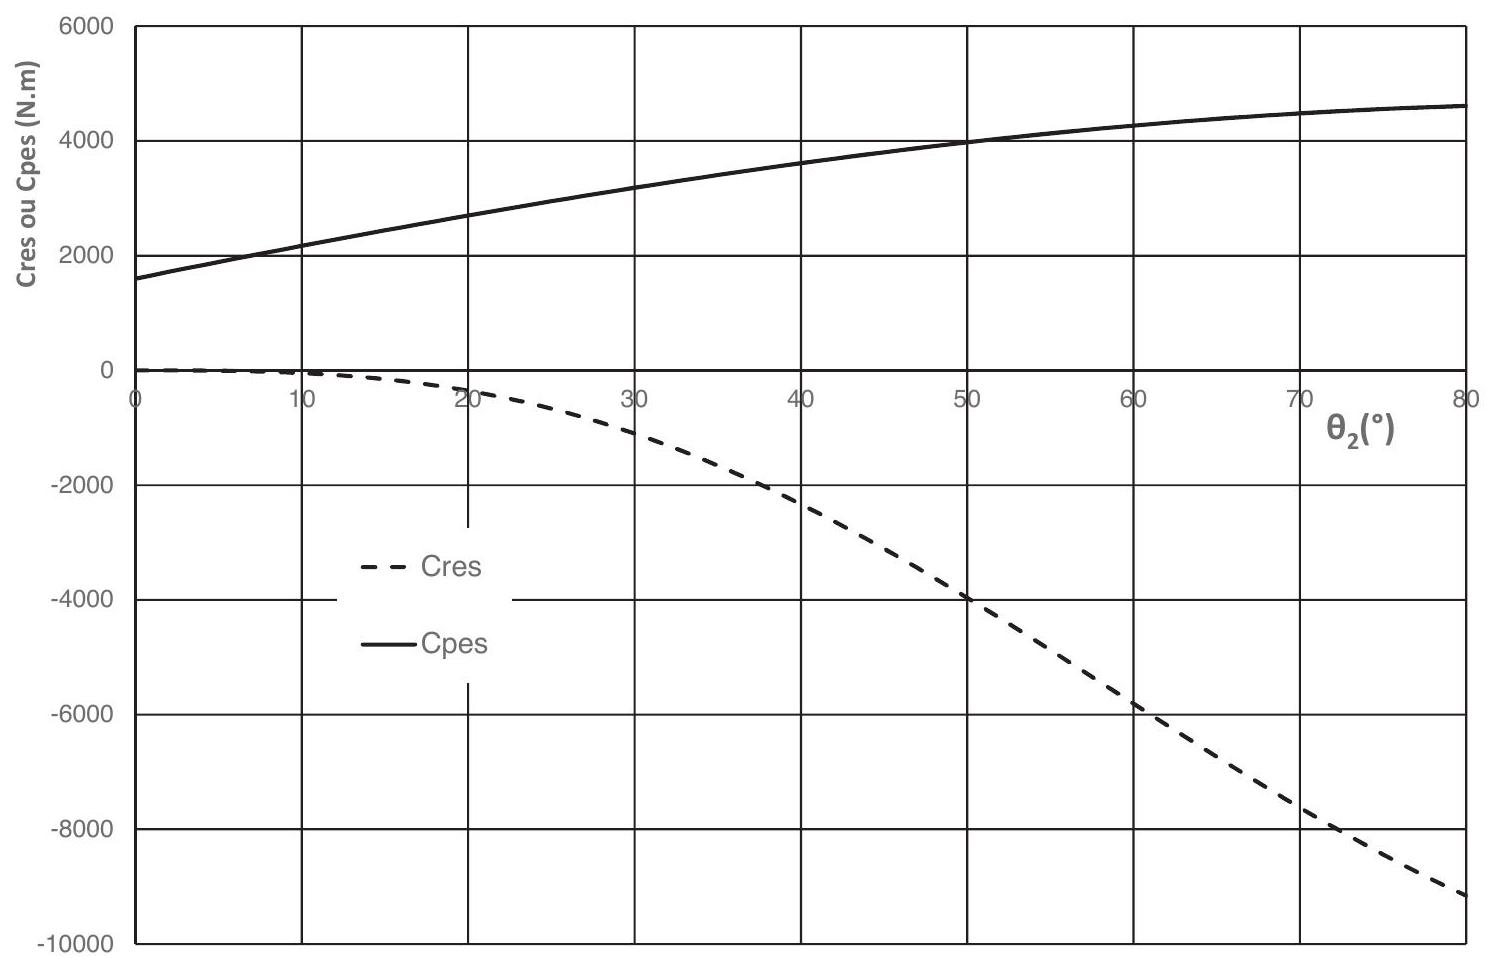
\includegraphics[width=.7\textwidth]{2023_11_27_dfbf12e0af72c49ac6a4g-10}
%Figure 9 - 
\caption{Evolution de $C_{\text{res}}$ et de $\indice{C}{pes}$ en fonction de $\theta_{2}$ \label{fig:09}}
\end{figure}


\question{\label{q:15}Indiquer la plage de valeurs de $\theta_{2}$ qui permet au dispositif d'équilibrage une compensation supérieure à $100 \%$ des effets de la gravité. En déduire si pour cette plage de valeurs, l'action du motoréducteur de l'axe $J_{2}$ du robot sera frein ou moteur si on néglige les effets d'inertie.}

\subsection{Étude du système articulé}
Le paramétrage et les caractéristiques de masses et d'inerties des différents sous-ensembles cinématiquement liés sont donnés en Annexe D.2.

L'objectif de cette partie est de déterminer l'expression des couples qui doivent être exercés par les motoréducteurs d'une part entre la base 1 et le bras 2 autour de l'axe $J_{2}\left(A, \vec{y}_{1}\right)$, et d'autre part entre les bras 2 et 3 autour de l'axe $J_{3}\left(B, \vec{y}_{1}\right)$ (voir Annexe D.1).

\section*{Pour la suite l'ensemble \{bras 3 ; masse ponctuelle $\}$ sera noté ensemble 4 .}
\begin{itemize}
  \item On considère que l'ensemble poignet, préhenseur et chargement est représenté par une masse ponctuelle $m_{E}$ en $E$.

  \item On note $G_{4}$ le centre d'inertie de l'ensemble 4 tel que $\overrightarrow{B G_{4}}=a_{4} \cdot \vec{z}_{3}-b_{4} \cdot \vec{x}_{3}$, et $m_{4}$ la masse de cet ensemble telle que $m_{4}=m_{3}+m_{E}$.

  \item On donne la représentation de l'opérateur d'inertie de l'ensemble 4 en $B$ dans la base $\mathcal{B}_{3}$ :
$
\mathbb{I}(B, 4)=\left[\begin{array}{ccc}
A_{4} & 0 & -E_{4} \\
0 & B_{4} & 0 \\
-E_{4} & 0 & C_{4}
\end{array}\right]_{\mathcal{B}_{3}}
$.
\end{itemize}

\question{Tracer le graphe de liaisons.}


\question{\label{q:16}Donner les expressions de $A_{4}, B_{4}, C_{4}$ et $E_{4}$ en fonction de $A_{3}, B_{3}, C_{3}, E_{3}, m_{E}$ et $L_{3}$.}

\question{\label{q:17}Définir la position du centre d'inertie $G_{4}$ en donnant les expressions de $a_{4}$ et $b_{4}$ en fonction de $a_{3}$, $m_{3}, m_{E}, L_{3}$ et $b_{3}$.}

On donne les torseurs modélisant les actions mécaniques du bras 2 sur le bras 3 et de la base 1 sur le bras 2 :

$\torseurstat{T}{2}{3}=\left\{\begin{array}{c}\vec{R}_{2 \rightarrow 3}=X_{23} \cdot \vec{x}_{0}+Y_{23} \cdot \vec{y}_{0}+Z_{23} \cdot \vec{z}_{0} \\ \vec{M}_{(B, 2 \rightarrow 3)}=L_{23} \cdot \vec{x}_{0}+C_{m 3} \cdot \vec{y}_{0}+N_{23} \cdot \vec{z}_{0}\end{array}\right\} ; \torseurstat{T}{1}{2}=\left\{\begin{array}{c}\vec{R}_{1 \rightarrow 2}=X_{12} \cdot \vec{x}_{0}+Y_{12} \cdot \vec{y}_{0}+Z_{12} \cdot \vec{z}_{0} \\ \vec{M}_{(A, 1 \rightarrow 2)}=L_{12} \cdot \vec{x}_{0}+C_{m 2} \cdot \vec{y}_{0}+N_{12} \cdot \vec{z}_{0}\end{array}\right\}$.


%\question{\label{q:18}Donner l'expression du vecteur vitesse $\vec{V}_{(B, 4 / 0)}$, puis du vecteur vitesse $\vec{V}_{\left(G_{4}, 4 / 0\right)}$.}


\question{\label{q:18a}Donner l'expression du vecteur vitesse $\vec{V}_{(B, 4 / 0)}$.}

\question{\label{q:18}Donner l'expression du vecteur vitesse $\vec{V}_{\left(G_{4}, 4 / 0\right)}$.}

\question{\label{q:19}Donner l'expression du moment cinétique $\vec{\sigma}_{(B, 4 / 0)}$.}

\question{\label{q:20}En déduire l'expression du moment dynamique $\vec{\delta}_{(B, 4 / 0)} \cdot \vec{y}_{0}$.}

\question{\label{q:21}Appliquer le théorème du moment dynamique à l'ensemble 4 en projection sur $\vec{y}_{0}$ de manière à donner l'expression du couple $C_{m 3}$ en fonction des angles $\theta_{2}, \theta_{3}$ et de leurs dérivées première et seconde, de $m_{4}$, et du moment d'inertie $B_{4}$.}

\question{\label{q:22}Donner l'expression du moment dynamique $\vec{\delta}_{(A, 2 / 0)}$.}

\question{\label{q:23}Sans calcul, donner la démarche pour déterminer l'expression du couple $C_{m 2}$.}
%
%\section*{C.3 Finalisation du modèle}
%Le modèle de comportement du système n'est pas linéaire car l'influence des charges et de l'action du système de compensation de pesanteur varie à chaque instant en fonction de $\theta_{2}$ et $\theta_{3}$.
%
%Un raisonnement sur des petits déplacements est effectué pour mettre en place une stratégie de correction qui évoluera en fonction de la position des bras.
%
%On se place dans une position particulière $z=z_{0}=364 \mathrm{~mm}$ lorsque $\theta_{2}=\theta_{20}=0^{\circ}$ et $\theta_{3}=\theta_{30}=123^{\circ}$. La charge se déplace suivant l'axe vertical d'une amplitude $\delta_{z}(t)$ qui correspond à des variations angulaires $\delta \theta_{2}(t)$ et $\delta \theta_{3}(t)$ au niveau des articulations. La vitesse initiale est nulle.
%
%Les équations linéarisées autour de cette position donnent :
%
%$$
%\begin{aligned}
%& \delta C_{m 2}=-\delta C_{r e s}+G_{0} \cdot \delta \theta_{2}+G_{1} \cdot \delta \theta_{3}+G_{2} \cdot \delta \ddot{\theta}_{2}+G_{3} \cdot \delta \ddot{\theta}_{3} \\
%& \delta C_{m 3}=G_{4} \cdot\left(\delta \theta_{2}+\delta \theta_{3}\right)+G_{5} \cdot \delta \ddot{\theta}_{2}+G_{6} \cdot \delta \ddot{\theta}_{3}
%\end{aligned}
%$$
%
%$$
%\begin{aligned}
%\text { avec } G_{0} & =-\left[m_{4} \cdot\left(L_{2} \cdot \cos \left(\theta_{20}\right)+a_{4} \cdot \cos \left(\theta_{20}+\theta_{30}\right)+b_{4} \cdot \sin \left(\theta_{20}+\theta_{30}\right)\right)+m_{2} \cdot a_{2} \cdot \cos \left(\theta_{20}\right)\right] \cdot g \\
%G_{1} & =-m_{4} \cdot\left(a_{4} \cdot \cos \left(\theta_{20}+\theta_{30}\right)+b_{4} \cdot \sin \left(\theta_{20}+\theta_{30}\right)\right) \cdot g \\
%G_{2} & =B_{2}+B_{4}+L_{2}^{2} \cdot m 4+2 \cdot L_{2} \cdot m_{4} \cdot\left(a_{4} \cdot \cos \left(\theta_{30}\right)+b_{4} \cdot \sin \left(\theta_{30}\right)\right) \\
%G_{3} & =B_{4}+L_{2} \cdot m_{4} \cdot\left(a_{4} \cdot \cos \left(\theta_{30}\right)+b_{4} \cdot \sin \left(\theta_{30}\right)\right) \\
%G_{4} & =-m_{4} \cdot\left(a_{4} \cdot \cos \left(\theta_{20}+\theta_{30}\right)+b_{4} \cdot \sin \left(\theta_{20}+\theta_{30}\right)\right) \cdot g \\
%G_{5} & =B_{4}+m_{4} \cdot L_{2} \cdot\left(a_{4} \cdot \cos \left(\theta_{30}\right)+b_{4} \cdot \sin \left(\theta_{30}\right)\right) \\
%G_{6} & =B_{4}
%\end{aligned}
%$$
%
%\begin{center}
%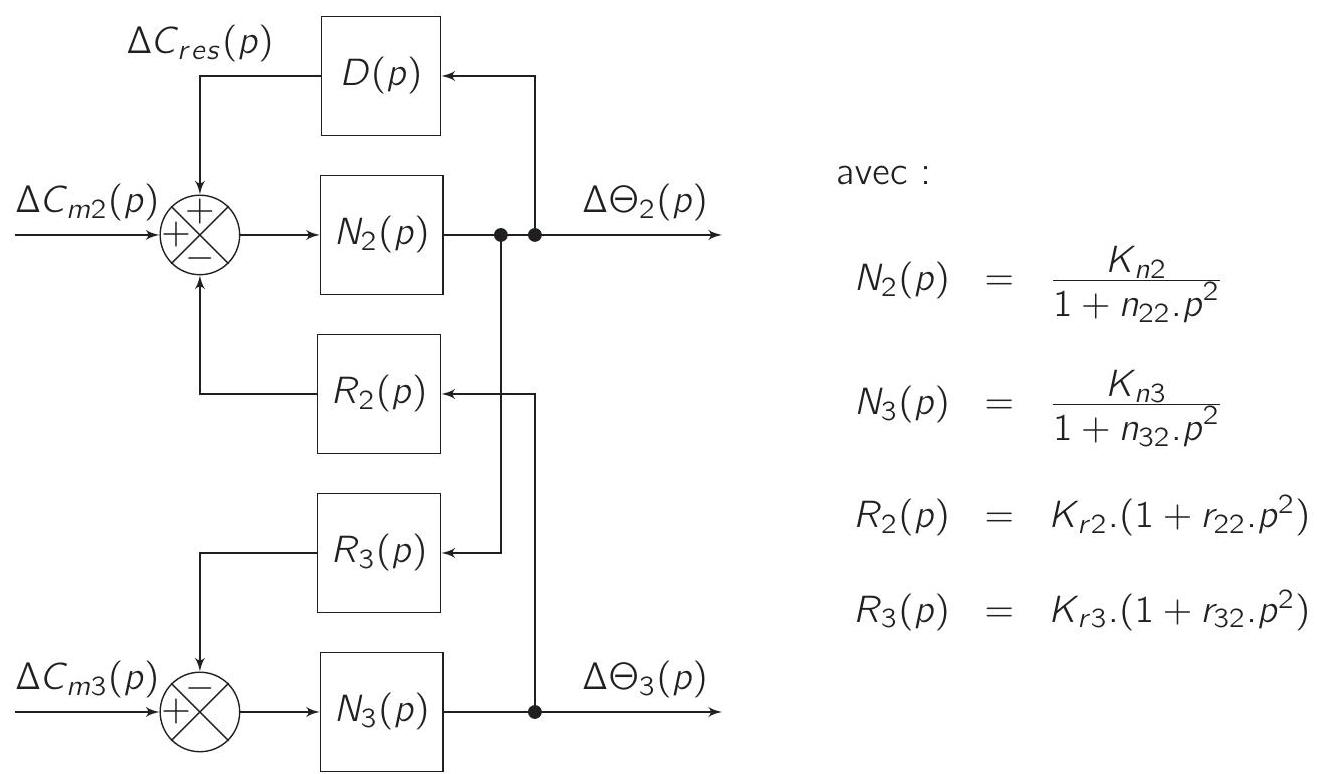
\includegraphics[max width=\textwidth]{2023_11_27_dfbf12e0af72c49ac6a4g-12(1)}
%\end{center}
%
%Figure $\mathbf{1 0}$ - Modèle de comportement du système articulé
%
%Le schéma bloc Figure $\mathbf{1 0}$ modélise le comportement dynamique du système articulé.
%
%On note $\Delta C_{m 2}(p), \Delta C_{m 3}(p), \Delta C_{\text {res }}(p), \Delta \Theta_{2}(p)$ et $\Delta \Theta_{3}(p)$ les transformées de Laplace respectives des fonctions temporelles $\delta C_{m 2}(t), \delta C_{m 3}(t), \delta C_{\text {res }}(t), \delta \theta_{2}(t)$ et $\delta \theta_{3}(t)$.
%
%Q24- Donner les expressions des coefficients $K_{n i}, n_{i 2}, K_{r i}$ et $r_{i 2}$ (avec $i=2$ ou 3) des fonctions de transferts $N_{2}(p), N_{3}(p), R_{2}(p)$ et $R_{3}(p)$ en fonction des coefficients $G_{j}(j=0$ à 6$)$.
%
%\begin{center}
%\includegraphics[max width=\textwidth]{2023_11_27_dfbf12e0af72c49ac6a4g-12}
%\end{center}
%
%\section*{Recherche d'une correction adaptée}
%Chaque axe est mis en mouvement par un moteur brushless dédié, associé à un réducteur permettant d'exercer les couples $C_{m 2}$ et $C_{m 3}$.
%
%Chaque moteur est piloté par un variateur qui permet de l'asservir en couple (donc en courant), en vitesse et/ou en position. Les variateurs utilisés permettent d'apporter une correction proportionnelle, intégrale et/ou dérivée (PID) sur chaque boucle. La mise en place de la boucle de courant, après correction, permet de simplifier le modèle de comportement du motoréducteur et donc d'aboutir à la simplification donnée par le schéma bloc Figure 11, modélisant le comportement de l'asservissement en position du système articulé. Les motoréducteurs utilisés pour les axes $J_{2}$ et $J_{3}$ (voir Annexe D.1) sont identiques.

\subsection*{Annexes}

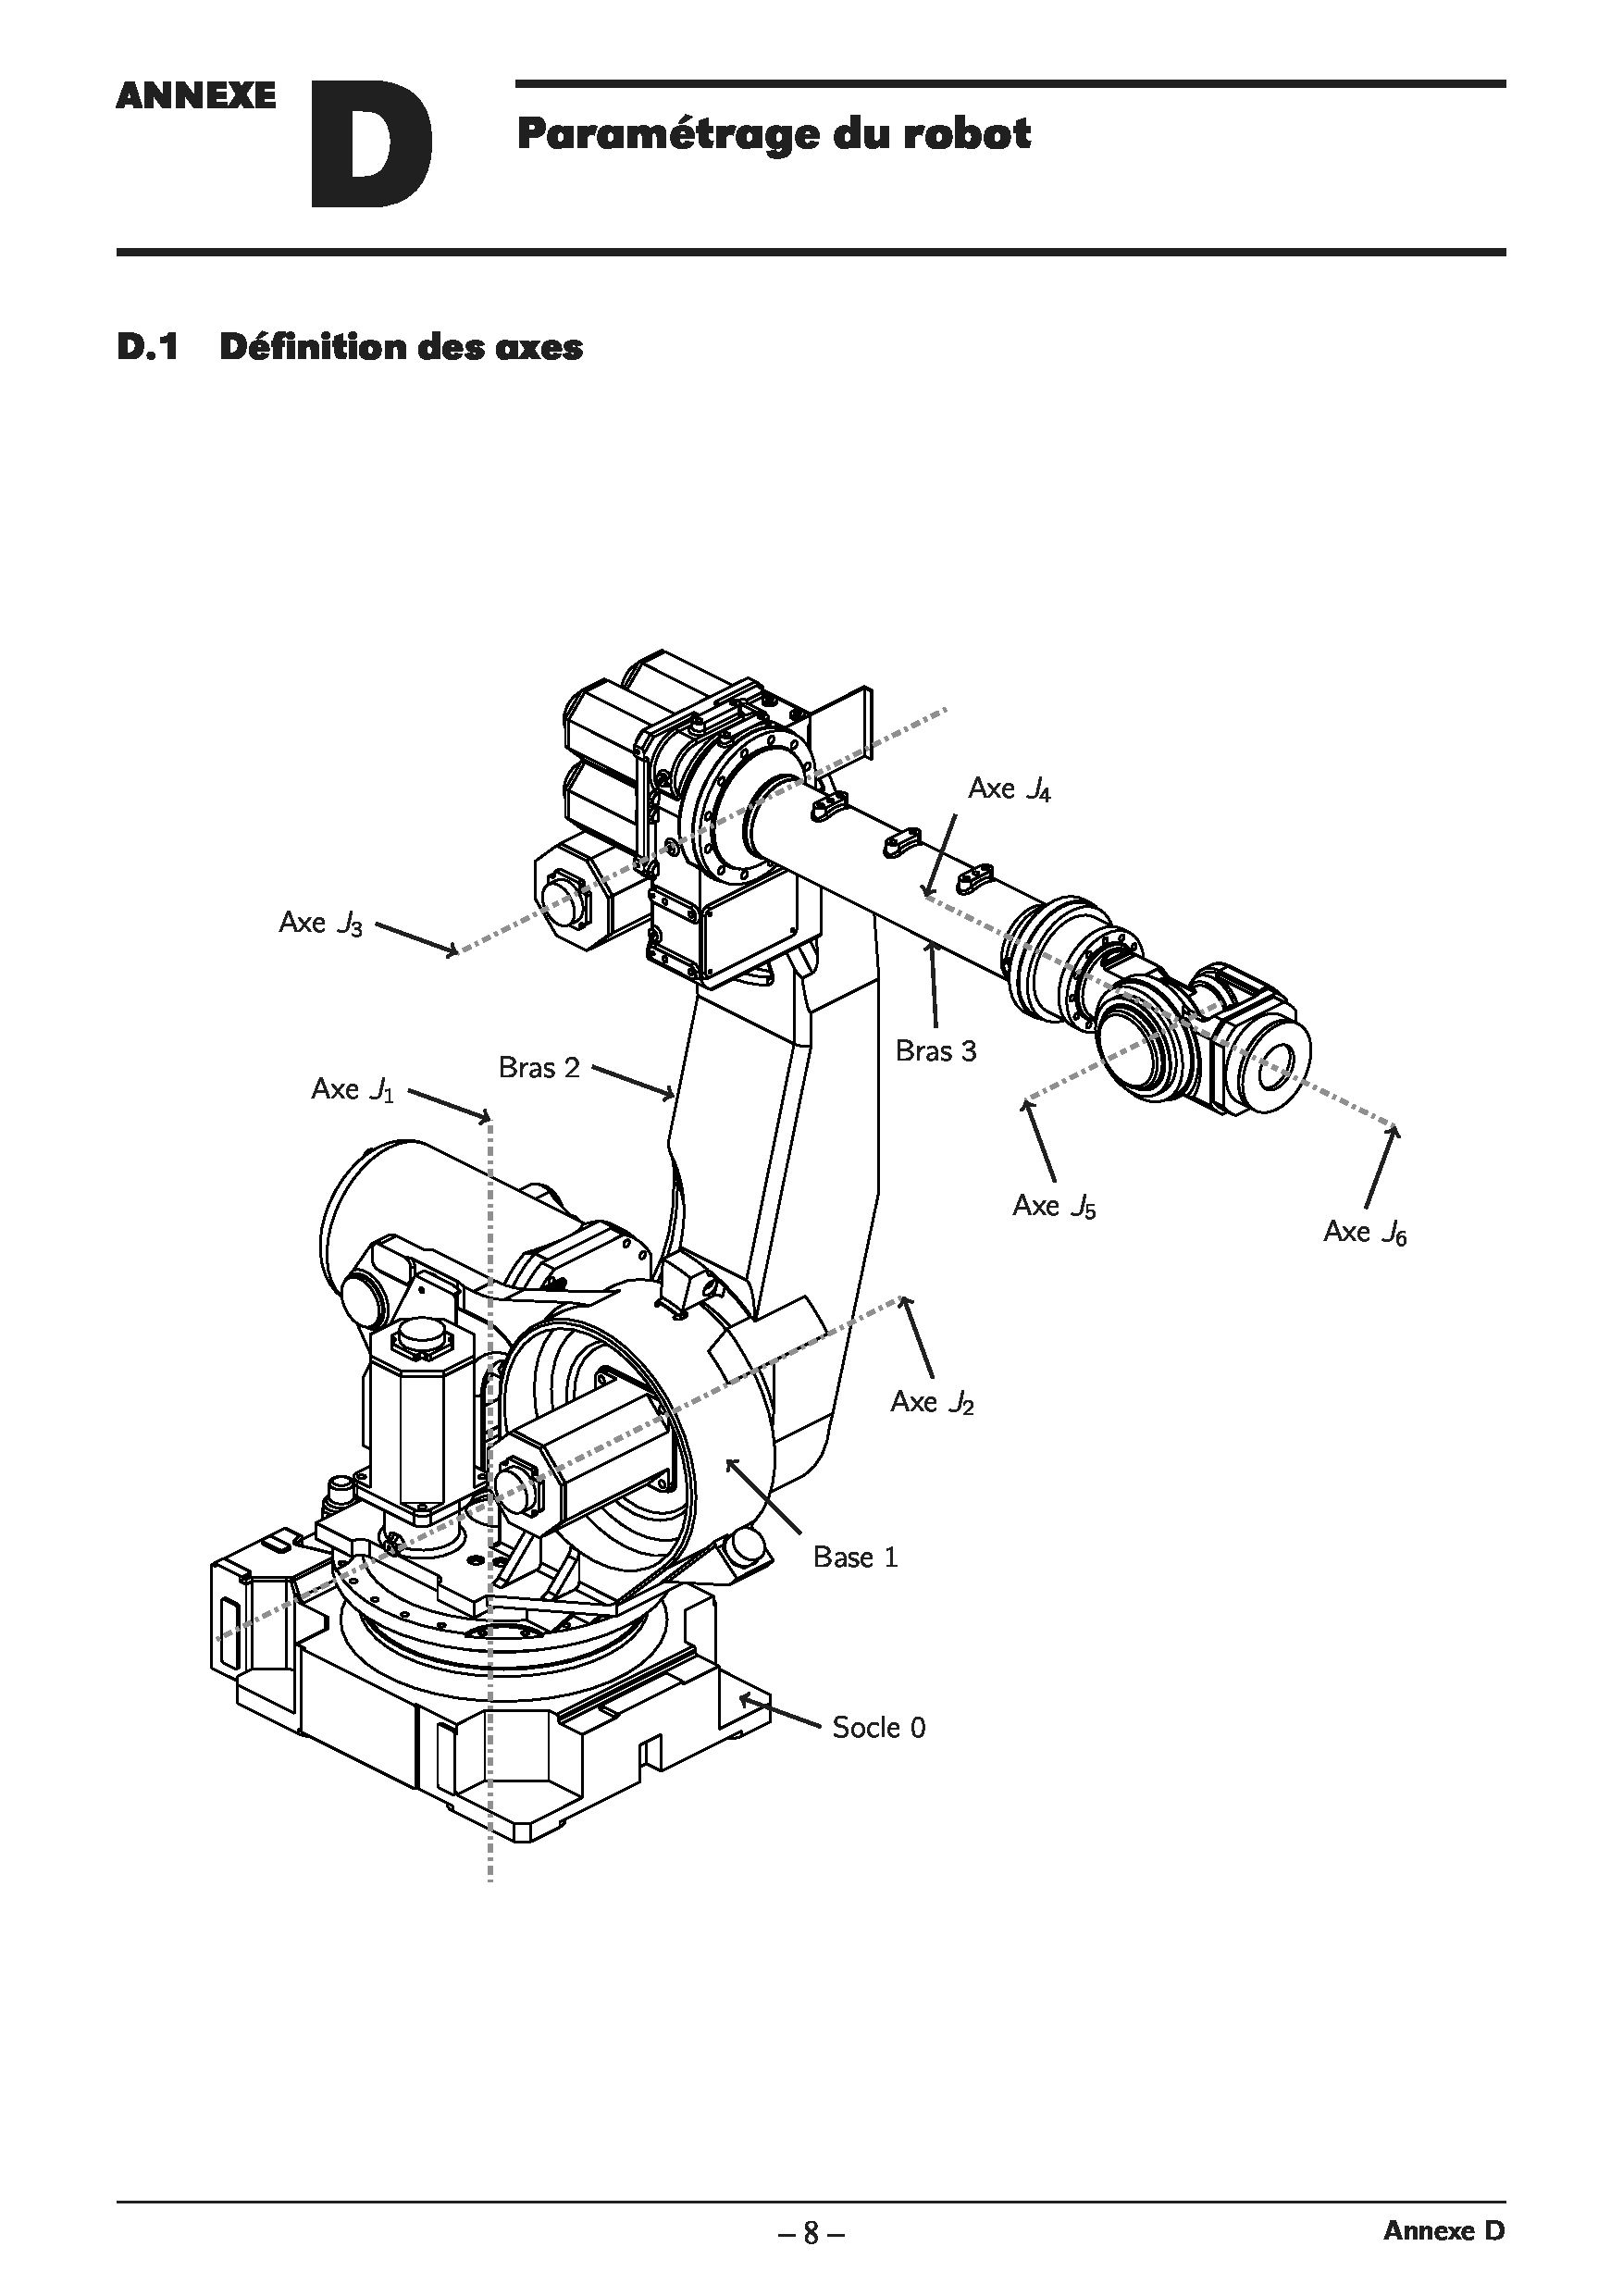
\includegraphics[width=\textwidth]{annexes}

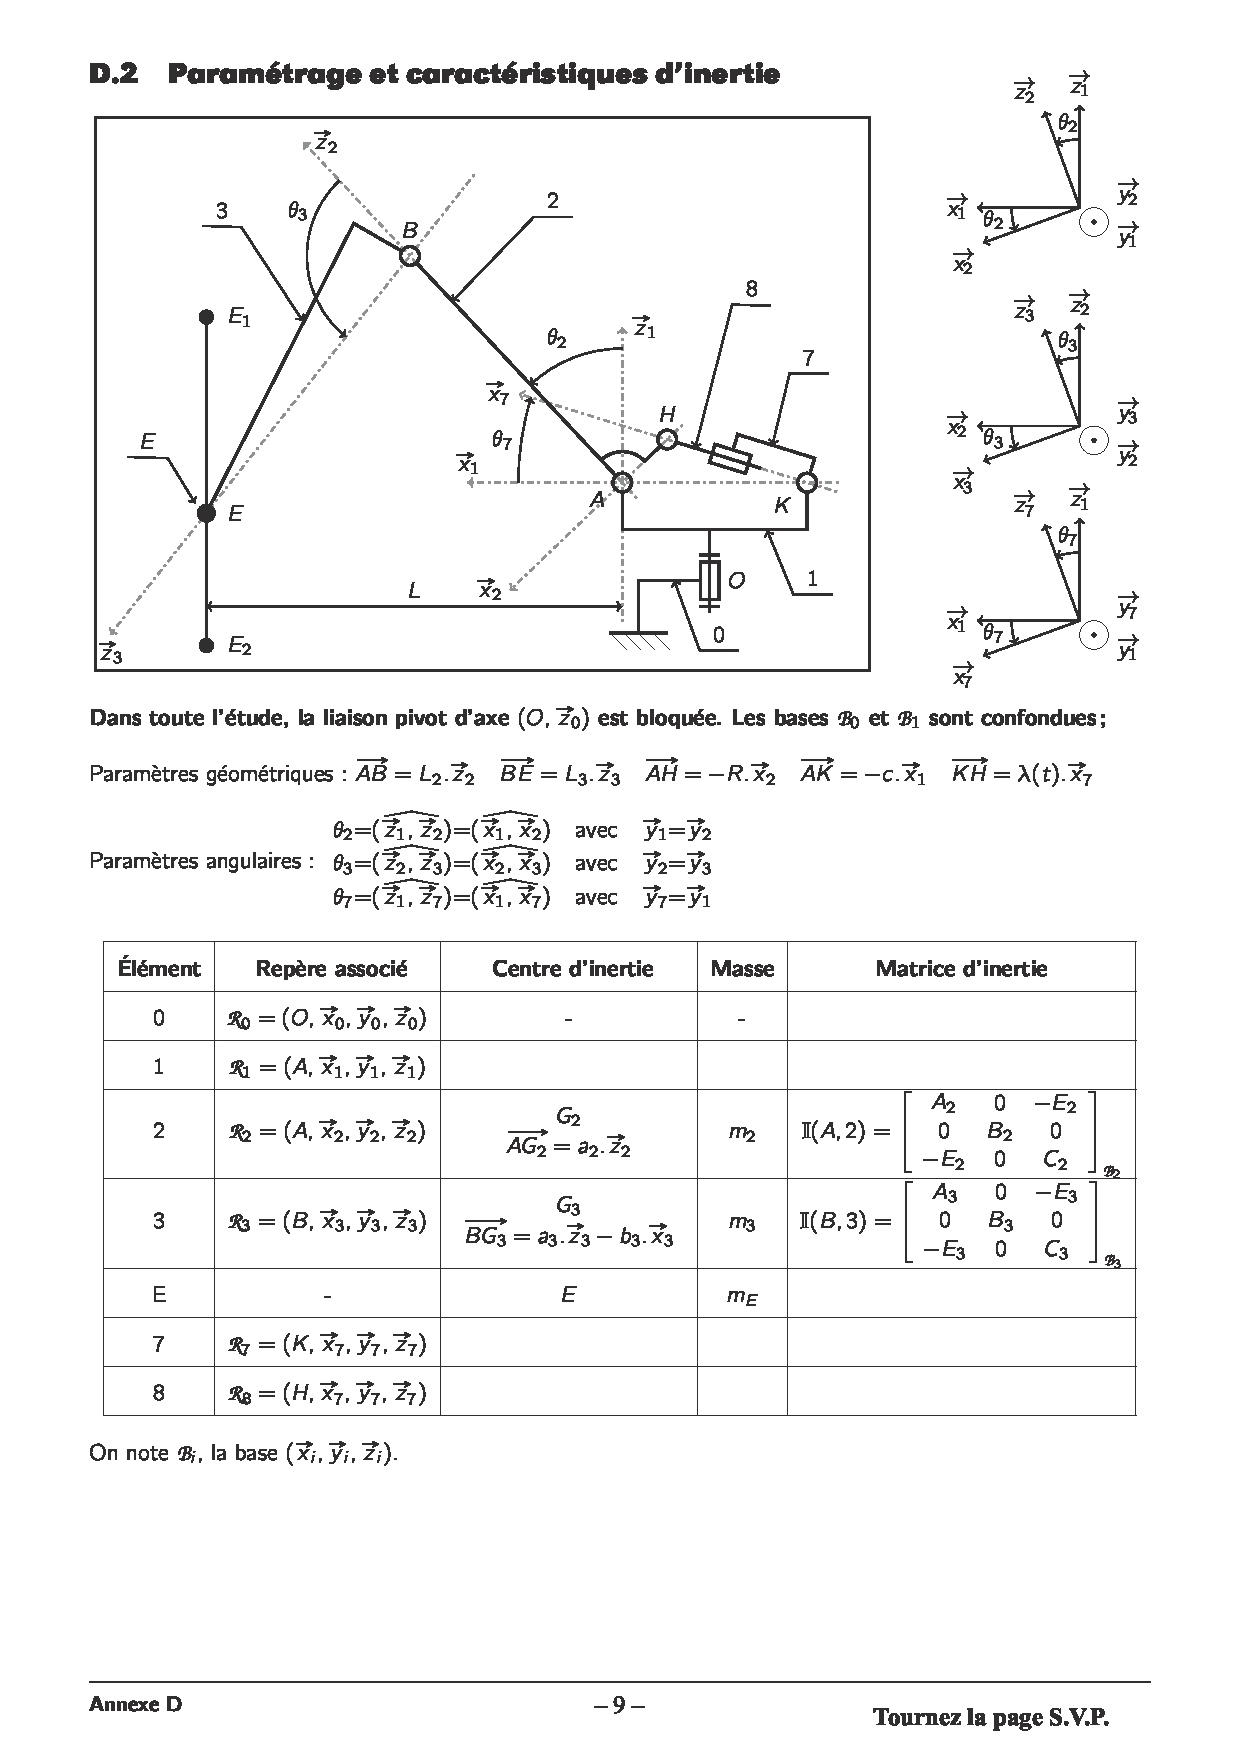
\includegraphics[width=\textwidth]{annexes2}

%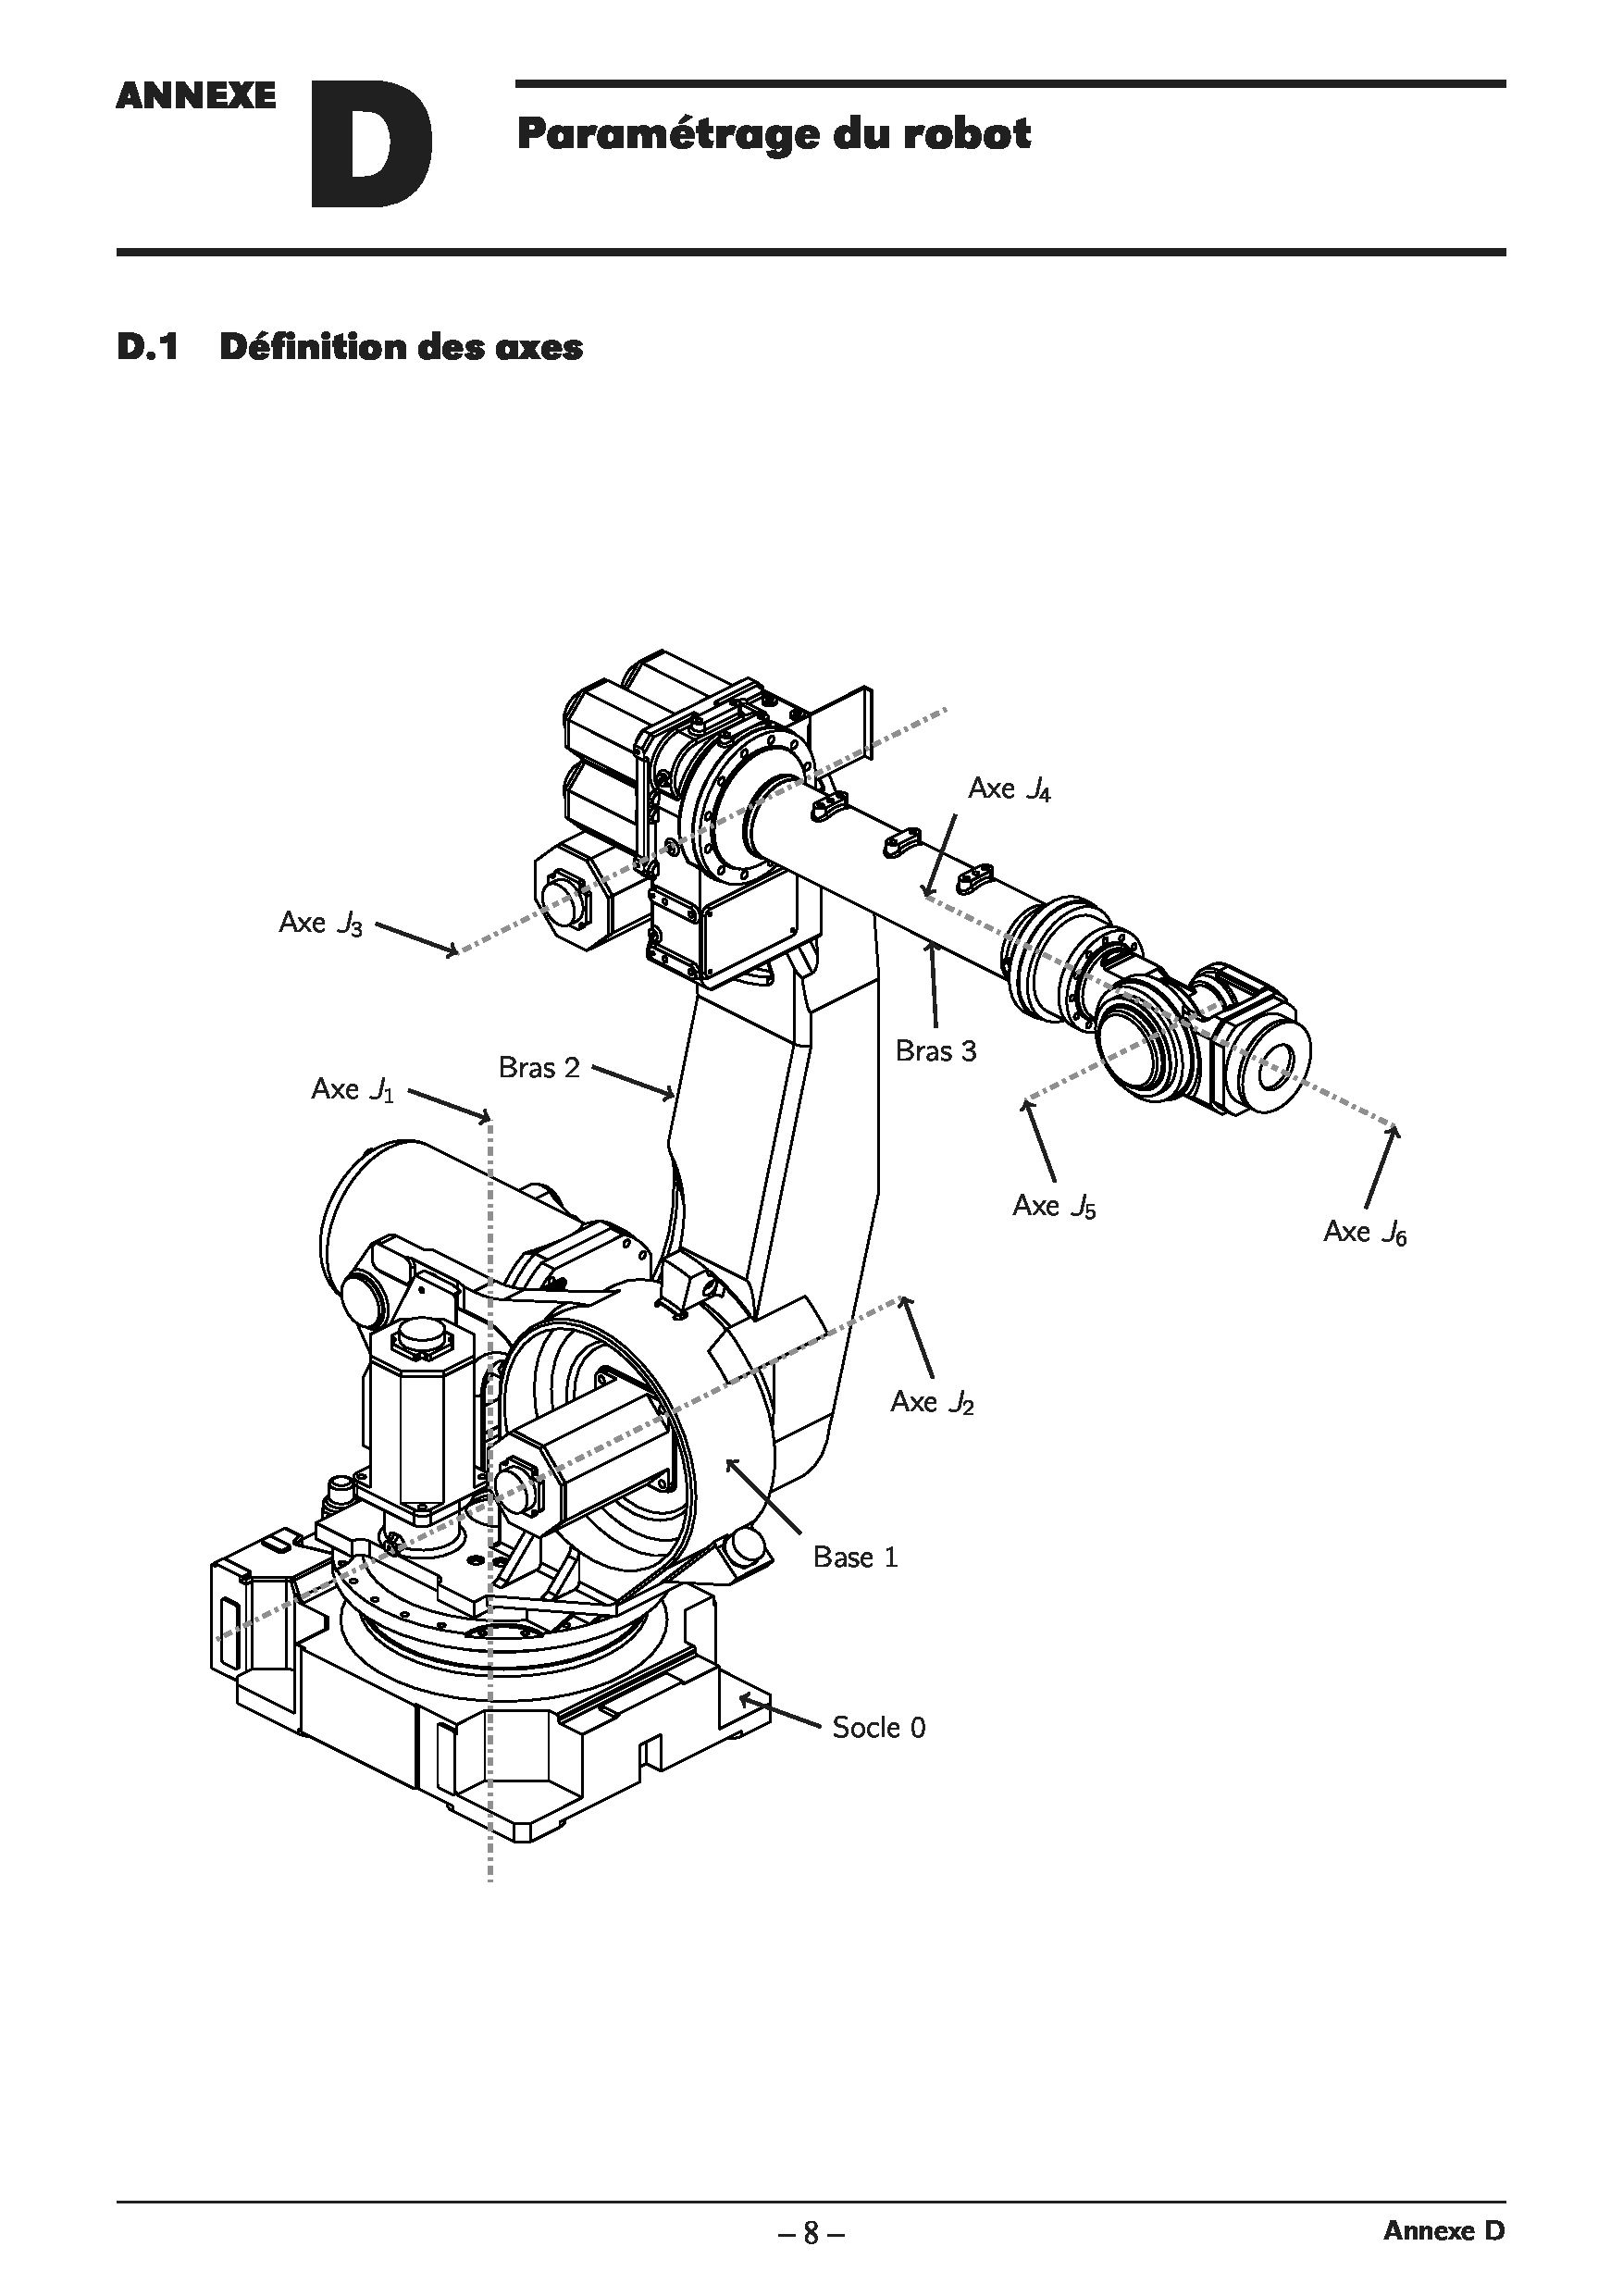
\includepdf[pages=-]{annexes.pdf}

\end{document}